\documentclass[a4paper, 12pt]{article}

% packages
\usepackage{amssymb}
\usepackage[fleqn]{mathtools}
\usepackage{tikz}
\usepackage{enumerate}
\usepackage{bussproofs}
\usepackage{xcolor}
\usepackage[margin=1.3cm]{geometry}
\usepackage{logicproof}
\usepackage{diagbox}
\usepackage{listings}
\usepackage{graphicx}
\usepackage{lstautogobble}
\usepackage{hyperref}
\usepackage{multirow}
\usepackage{tipa}
\usepackage{pgfplots}
\usepackage{adjustbox}

% tikz libraries
\usetikzlibrary{
    decorations.pathreplacing,
    arrows,
    shapes,
    shapes.gates.logic.US,
    circuits.logic.US,
    calc,
    automata,
    positioning,
    intersections
}

\pgfplotsset{compat=1.16}

\pgfmathdeclarefunction{gauss}{2}{%
  \pgfmathparse{1/(#2*sqrt(2*pi))*exp(-((x-#1)^2)/(2*#2^2))}%
}

\allowdisplaybreaks % allow environments to break
\setlength\parindent{0pt} % no indent

% shorthand for verbatim
% this clashes with logicproof, so maybe fix this at some point?
\catcode`~=\active
\def~#1~{\texttt{#1}}

% code listing
\lstdefinestyle{main}{
    numberstyle=\tiny,
    breaklines=true,
    showspaces=false,
    showstringspaces=false,
    tabsize=2,
    numbers=left,
    basicstyle=\ttfamily,
    columns=fixed,
    fontadjust=true,
    basewidth=0.5em,
    autogobble,
    xleftmargin=3.0ex,
    mathescape=true
}
\newcommand{\dollar}{\mbox{\textdollar}} %
\lstset{style=main}

% augmented matrix
\makeatletter
\renewcommand*\env@matrix[1][*\c@MaxMatrixCols c]{%
\hskip -\arraycolsep
\let\@ifnextchar\new@ifnextchar
\array{#1}}
\makeatother

% ceiling / floor
\DeclarePairedDelimiter{\ceil}{\lceil}{\rceil}
\DeclarePairedDelimiter{\floor}{\lfloor}{\rfloor}

% custom commands
\newcommand{\indefint}[2]{\int #1 \, \mathrm{d}#2}
\newcommand{\defint}[4]{\int_{#1}^{#2} #3 \, \mathrm{d}#4}
\newcommand{\pdif}[2]{\frac{\partial #1}{\partial #2}}
\newcommand{\dif}[2]{\frac{\mathrm{d}#1}{\mathrm{d}#2}}
\newcommand{\limit}[2]{\raisebox{0.5ex}{\scalebox{0.8}{$\displaystyle{\lim_{#1 \to #2}}$}}}
\newcommand{\limitsup}[2]{\raisebox{0.5ex}{\scalebox{0.8}{$\displaystyle{\limsup_{#1 \to #2}}$}}}
\newcommand{\summation}[2]{\sum\limits_{#1}^{#2}}
\newcommand{\product}[2]{\prod\limits_{#1}^{#2}}
\newcommand{\intbracket}[3]{\left[#3\right]_{#1}^{#2}}
\newcommand{\laplace}{\mathcal{L}}
\newcommand{\fourier}{\mathcal{F}}
\newcommand{\mat}[1]{\boldsymbol{#1}}
\renewcommand{\vec}[1]{\boldsymbol{#1}}
\newcommand{\rowt}[1]{\begin{bmatrix}
    #1
\end{bmatrix}^\top}
\DeclareMathOperator*{\argmax}{argmax}
\DeclareMathOperator*{\argmin}{argmin}

\newcommand{\lto}[0]{\leadsto\ }

\newcommand{\ulsmash}[1]{\underline{\smash{#1}}}

\newcommand{\powerset}[0]{\wp}
\renewcommand{\emptyset}[0]{\varnothing}

\makeatletter
\newsavebox{\@brx}
\newcommand{\llangle}[1][]{\savebox{\@brx}{\(\m@th{#1\langle}\)}%
  \mathopen{\copy\@brx\kern-0.5\wd\@brx\usebox{\@brx}}}
\newcommand{\rrangle}[1][]{\savebox{\@brx}{\(\m@th{#1\rangle}\)}%
  \mathclose{\copy\@brx\kern-0.5\wd\@brx\usebox{\@brx}}}
\makeatother
\newcommand{\lla}{\llangle}
\newcommand{\rra}{\rrangle}
\newcommand{\la}{\langle}
\newcommand{\ra}{\rangle}
\newcommand{\crnr}[1]{\text{\textopencorner} #1 \text{\textcorner}}
\newcommand{\bnfsep}[0]{\ |\ }
\newcommand{\concsep}[0]{\ ||\ }

\newcommand{\axiom}[1]{\AxiomC{#1}}
\newcommand{\unary}[1]{\UnaryInfC{#1}}
\newcommand{\binary}[1]{\BinaryInfC{#1}}
\newcommand{\trinary}[1]{\TrinaryInfC{#1}}
\newcommand{\quaternary}[1]{\QuaternaryInfC{#1}}
\newcommand{\quinary}[1]{\QuinaryInfC{#1}}
\newcommand{\dproof}[0]{\DisplayProof}
\newcommand{\llabel}[1]{\LeftLabel{\scriptsize #1}}
\newcommand{\rlabel}[1]{\RightLabel{\scriptsize #1}}

\newcommand{\ttbs}{\char`\\}
\newcommand{\lrbt}[0]{\ \bullet\ }

% colours
\newcommand{\violet}[1]{\textcolor{violet}{#1}}
\newcommand{\blue}[1]{\textcolor{blue}{#1}}
\newcommand{\red}[1]{\textcolor{red}{#1}}
\newcommand{\teal}[1]{\textcolor{teal}{#1}}

% reasoning proofs
\usepackage{ltablex}
\usepackage{environ}
\keepXColumns
\NewEnviron{reasoning}{
    \begin{tabularx}{\textwidth}{rlX}
        \BODY
    \end{tabularx}
}
\newcommand{\proofline}[3]{$(#1)$ & $#2$ & \hfill #3 \smallskip \\}
\newcommand{\proofarbitrary}[1]{& take arbitrary $#1$ \smallskip \\}
\newcommand{\prooftext}[1]{\multicolumn{3}{l}{#1} \smallskip \\}
\newcommand{\proofmath}[3]{$#1$ & = $#2$ & \hfill #3 \smallskip \\}
\newcommand{\prooftherefore}[1]{& $\therefore #1$ \smallskip \\}
\newcommand{\proofbc}[0]{\prooftext{\textbf{Base Case}}}
\newcommand{\proofis}[0]{\prooftext{\textbf{Inductive Step}}}

% ER diagrams
\newcommand{\nattribute}[4]{
    \node[draw, state, inner sep=0cm, minimum size=0.2cm, label=#3:{#4}] (#1) at (#2) {};
}
\newcommand{\mattribute}[4]{
    \node[draw, state, accepting, inner sep=0cm, minimum size=0.2cm, label=#3:{#4}] (#1) at (#2) {};
}
\newcommand{\dattribute}[4]{
    \node[draw, state, dashed, inner sep=0cm, minimum size=0.2cm, label=#3:{#4}] (#1) at (#2) {};
}
\newcommand{\entity}[3]{
    \node[] (#1-c) at (#2) {#3};
    \node[inner sep=0cm] (#1-l) at ($(#1-c) + (-1, 0)$) {};
    \node[inner sep=0cm] (#1-r) at ($(#1-c) + (1, 0)$) {};
    \node[inner sep=0cm] (#1-u) at ($(#1-c) + (0, 0.5)$) {};
    \node[inner sep=0cm] (#1-d) at ($(#1-c) + (0, -0.5)$) {};
    \draw
    ($(#1-c) + (-1, 0.5)$) -- ($(#1-c) + (1, 0.5)$) -- ($(#1-c) + (1, -0.5)$) -- ($(#1-c) + (-1, -0.5)$) -- cycle;
}
\newcommand{\relationship}[3]{
    \node[] (#1-c) at (#2) {#3};
    \node[inner sep=0cm] (#1-l) at ($(#1-c) + (-1, 0)$) {};
    \node[inner sep=0cm] (#1-r) at ($(#1-c) + (1, 0)$) {};
    \node[inner sep=0cm] (#1-u) at ($(#1-c) + (0, 1)$) {};
    \node[inner sep=0cm] (#1-d) at ($(#1-c) + (0, -1)$) {};
    \draw
    ($(#1-c) + (-1, 0)$) -- ($(#1-c) + (0, 1)$) -- ($(#1-c) + (1, 0)$) -- ($(#1-c) + (0, -1)$) -- cycle;
}

% AVL Trees
\newcommand{\avltri}[4]{
    \draw ($(#1)$) -- ($(#1) + #4*(0.5, -1)$) -- ($(#1) + #4*(-0.5, -1)$) -- cycle;
    \node at ($(#1) + #4*(0, -1) + (0, 0.5)$) {#3};
    \node at ($(#1) + #4*(0, -1) + (0, -0.5)$) {#2};
}

% RB Trees
\tikzset{rbtr/.style={inner sep=2pt, circle, draw=black, fill=red}}
\tikzset{rbtb/.style={inner sep=2pt, circle, draw=black, fill=black}}

% Samples
\tikzset{spos/.style={inner sep=2pt, circle, draw=black, fill=blue!20}}
\tikzset{sneg/.style={inner sep=2pt, circle, draw=black, fill=red!20}}

% Joins
\newcommand\ljoin{\stackrel{\mathclap{\normalfont\mbox{\tiny L}}}{\bowtie}}
\newcommand\rjoin{\stackrel{\mathclap{\normalfont\mbox{\tiny R}}}{\bowtie}}
\newcommand\ojoin{\stackrel{\mathclap{\normalfont\mbox{\tiny O}}}{\bowtie}}

\setcounter{MaxMatrixCols}{100}

% actual document
\begin{document}
    {\sc Computing $4^\text{th}$ Year Notes} \hfill ~https://github.com/lin-e/imperial-revision~
    \rule{\textwidth}{0.1pt}
    \section*{Scalable Systems and Data \hfill (70022)}
        \subsection*{1.1 - Database Storage Layer}
            This lecture covers the DBMS layers, storage hierarchy as well as the role disks takes in the DBMS.
            The DBMS layers are as follows, with the query going into the first layer, and storage being the final layer.
            Note that the last two layers (buffer management and disk space management are typically done by the OS).
            \begin{enumerate}[1.]
                \itemsep0em
                \item \textbf{query optimization and execution} \hfill tries to reorganise the query to execute efficiently
                \item \textbf{relational operators}
                \item \textbf{file and access methods} \hfill understand which files need to be accessed and indexes we can use
                \item \textbf{buffer management} \hfill handles reading disk pages and buffering in main memory for fast access
                \item \textbf{disk space management}
            \end{enumerate}
            An example of this could be a search engine, which is much simpler than a general DBMS - albeit having similar layers;
            \begin{enumerate}[1.]
                \itemsep0em
                \item search string modifier
                \item ranking engine
                \item query execution
                \item buffer management
                \item disk space management
            \end{enumerate}
            This is simpler than a DBMS as it can simply use the OS for the bottom two layers, there is typically no concurrency (nor any need for transactions, being mostly read-only), and typically has hard-wired queries.
            The ranking engine and query execution is a simple DBMS.
            \subsubsection*{DBMS versus Using OS}
                An important question is why we don't simply use the OS.
                The layers of abstractions can be useful, but we have a lot of knowledge on how to access the data.
                In addition, the OS can often get in the way of the DBMS - it has some idea on what to query and what files to touch, and knows more about the OS regarding future access, which can be exploited.
                A DBMS needs to do things its own way, for example specialised pre-fetching with the knowledge of future access.
                Additionally, if we control the buffer management, we can also control the replacement policy, likely with something better than the OS.
                With more control over the thread / process scheduling, the DBMS can achieve a more optimal execution of the workflow as the DB locks aren't going to conflict with the OS locks (high contention).
                There's also control over flushing data to the disk, including writing log file (important for recovery), and shouldn't be left to the OS.
            \subsubsection*{Disks and Files}
                Today, disks are still the go-to storage medium for large amounts of files, and have become fairly affordable (not as affordable as tape for archival storage, but much cheaper than other media, such as SSD or main memory).
                Unlike other media, disks have mechanical parts leading to differences access patterns or behaviour - the time to access a piece of data is affected by \textbf{where} the data is on the disk.
                A lot of databases today are still on disks, as it's cheap with a reasonable access time - typically the data is read from the disk onto main memory (buffered), and changes are written back to the disk from the buffer.
                \medskip

                High-end databases are in the petabyte range, therefore using main memory would be extremely expensive.
                In addition to that, main memory is volatile - meaning the data is lost if power goes out.
                However, main-memory databases do exist for smaller sized, performance optimised systems, in which volatility is tolerable.
                \medskip

                Flash storage isn't commonly used in DBMS as main storage (due to the cost), but can also be used as an accelerator or enabler, in the form of a specialised cache, etc.
                \medskip

                The storage hierarchy is as follows.
                Note that flash storage can either be used to the side of magnetic disk (for a specific portion of the files), or as a buffer on top (before main memory).
                \textit{Jim Gray} has an analogy for how far away the data is (registers being knowledge in your head, etc), illustrating the scale of access time.
                \begin{center}
                    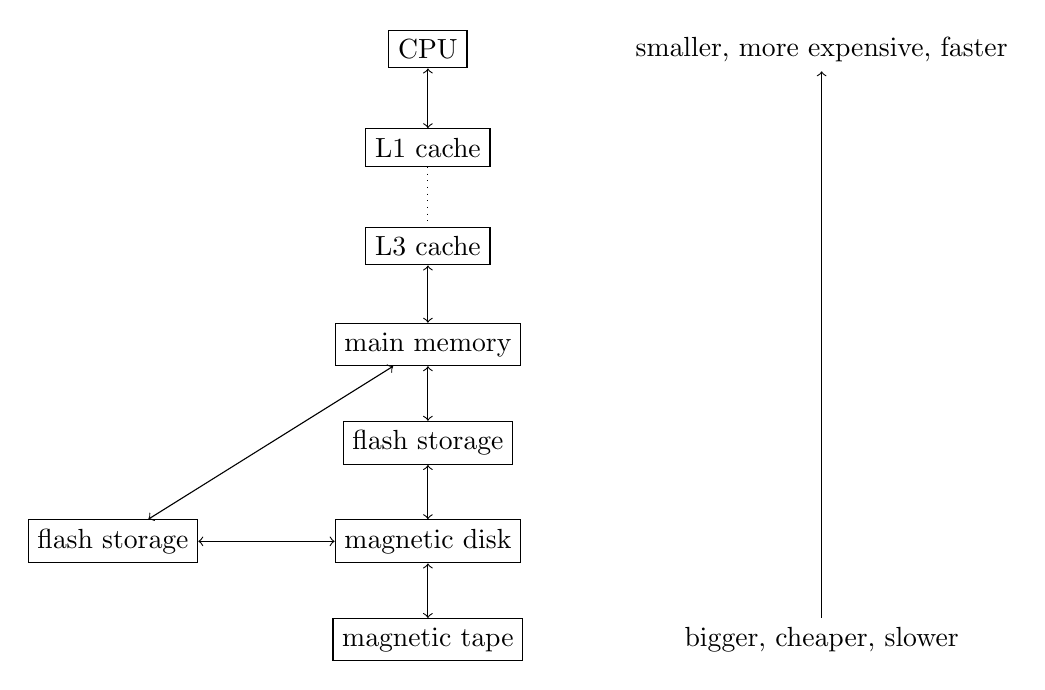
\begin{tikzpicture}[y=1.25cm]
                        \node[draw] (cpu) at (0, 0) {CPU};
                        \node[draw] (l1) at (0, -1) {L1 cache};
                        \node[draw] (l3) at (0, -2) {L3 cache};
                        \node[draw] (mm) at (0, -3) {main memory};
                        \node[draw] (fs1) at (0, -4) {flash storage};
                        \node[draw] (md) at (0, -5) {magnetic disk};
                        \node[draw] (fs2) at (-4, -5) {flash storage};
                        \node[draw] (mt) at (0, -6) {magnetic tape};

                        \draw
                        (cpu) edge[<->] (l1)
                        (l1) edge[dotted] (l3)
                        (l3) edge[<->] (mm)
                        (mm) edge[<->] (fs1)
                        (mm) edge[<->] (fs2)
                        (fs1) edge[<->] (md)
                        (fs2) edge[<->] (md)
                        (md) edge[<->] (mt);

                        \node (x) at (5, -6) {bigger, cheaper, slower};
                        \node (y) at (5, 0) {smaller, more expensive, faster};

                        \draw (x) edge[->] (y);
                    \end{tikzpicture}
                \end{center}
                Disks are still the main secondary storage device of choice, with the main advantage over tapes being the ability to perform random access, rather than purely sequential.
                Data is stored in units in \textbf{disk blocks} or \textbf{pages} (may be used interchangeably), typically in the order of kilobytes and occasionally megabytes.
                Unlike RAM, the time to retrieve / write a disk page varies depending on the location, with a tremendous impact on time to retrieve, hence relative placement of pages on a disk has a major impact on performance.
                The lecture then goes over the anatomy of a disk;
                \begin{itemize}
                    \itemsep0em
                    \item spindle and platters spin between 5,000 - 15,000 RPM (with physical limitations)
                    \item arm assembly has multiple disk head, one for each platter - the tracks under the heads form a cylinder
                    \item only one head reads or writes at once
                \end{itemize}
                The time to access a disk block has three elements;
                \begin{itemize}
                    \itemsep0em
                    \item \textbf{seek time} \hfill time to move the arm to the correct position (in and out, towards the spindle)
                    \item \textbf{rotational delay} \hfill arm assembly in a fixed position, block needs to be rotated under head
                    \item \textbf{transfer time} \hfill actual time to read data from disk into main memory
                \end{itemize}
                The time for a smaller number of cylinders traversed is dominated by the seek time (head positioning).
                In modern disks, short seeks are dominated by the \textbf{settle time}, which gets larger with increased disk track density.
                \medskip

                Generally, the seek time and rotational delay dominates, with the former being in the range of 1 to 20ms, and the latter being in the range of 0 to 10ms.
                On the other hand, the transfer rate is less than 1 millisecond for a 4KB page.
                As such, the key to lower I/O cost is to reduce the delays caused by seek and rotation.
                Additionally, in shared disks, most of the time is spent waiting for access to the arm.
                \medskip

                The concept of the next block is as follows;
                \begin{itemize}
                    \itemsep0em
                    \item blocks on the same track, followed by
                    \item blocks on the same cylinder
                    \item blocks on adjacent cylinder
                \end{itemize}
                We can't control where we write on the disk - that's controlled by the device driver.
                Typically, if data is written together, it will also be read together.
                Defragmentation is disk optimization, as data can be spread out all over a disk for a given file, leading to slower read times - this is done by putting all the pieces of a file closer together.
                \medskip

                Note that an adjacent block doesn't necessarily mean physically adjacent.
                Data can be physically spread out over a disk but in a certain pattern that can lead to near sequential access.
                The adjacent blocks can be the blocks under the disk head after rotating during settle time.
                \medskip

                In general, memory access is much faster than disk I/O (roughly $1,000 \times$), and sequential I/O is faster than random (roughly $10 \times$).
                \medskip

                The lowest layer of DBMS manages the space on the disk and higher levels can call this layer to allocate / de-allocate a page, or read / write a page.
            \subsubsection*{Summary}
                In general, the key for storing data on a disk is to store data together if it's queried together.
                Random access should be avoided, preferably use sequential access.
                Data structures should be aligned for page size - for example, if a data structure were to have a few bytes in the next page, an additional page would have to be retrieved, despite mostly being irrelevant.
        \subsection*{1.2 - Main Memory Indexing}
            The general trend is that we have more main memory as time goes on.
            The hardware trends show that CPU speed and main memory capacity doubles every 18 months, however memory speed only grows by 10\% per year.
            \medskip

            This means that many databases, typically OLTP, can fit into main memory; OLAP is still in the order of petabytes, if not more.
            Memory access has become the new bottleneck for main memory databases.
            There is no longer a uniform random access model (NUMA), meaning that we can no longer assume that accessing each piece of data in memory takes the same amount of time.
            Cache performance has become crucial.
            \medskip

            The memory hierarchy is as follows.
            Note that a cache \textbf{line} is the smallest unit that can be retrieved from the cache, and data structures should be aligned to a line in a similar way to pages.
            \begin{itemize}
                \itemsep0em
                \item CPU (registers)
                \item L1 cache, takes 1 cycle, 8-64 KB, 32 bytes per line
                \item L2 cache, takes 2 - 10 cycles, 64 - 128 bytes per line
                \item TLB, takes 10 - 100 cycles, 64 entries / pages
            \end{itemize}
            The cache performance is crucial, similar to the disk cache / buffer pool, however the DBMS doesn't have direct control of this.
            \subsubsection*{Improving Cache Performance}
                The primary factors are the cache capacity and data locality, the former is a given and can't be changed, whereas we can do something about the locality.
                An example with non-random access, such as a scan or index traversal is by clustering data structures to a multiple of a cache line, as well as squeezing more useful data into a cache line.
                On the other hand, with random access, such as in a hash join, the data should be partitioned to fit in cache / TLB.
                CPU is often also traded for memory access, such as compression (requires more CPU processing, but reduces storage usage).
            \subsubsection*{Trees}
                The lecture then goes through an example of a tree index, where each node holds 2 entries.
                Each node can point to three other nodes, where the values are either below, in between the two values, or higher than both.
                \medskip

                The B+ tree is quite similar, but all leaf nodes are connected.
                This allows for faster execution of range queries, as the nodes are connected without traversing up and down the tree.
                The \textbf{order} is the minimum number of keys or pointers in a non-leaf node and the \textbf{fanout} of a node is the number of pointers out of the node.
                These have the following properties;
                \begin{itemize}
                    \itemsep0em
                    \item balanced - leaves are at the same level, leading to predictable performance when traversing down the tree (same for every node)
                    \item every node, other than the root, must be at least half full meaning it becomes balanced
                    \item searching is $\log_d(n)$, where $d$ is the order and $n$ is the number of entries
                    \item insertion involves finding the leaf to insert to, splitting if the node is full and adjusting index accordingly; has a similar cost to searching, have to find all the way down, and may have to split all the way back up
                    \item deletion is similar, find leaf node, delete, and merge neighbouring nodes if required (not half-full)
                \end{itemize}
                \textbf{Cache sensitive search trees} can be thought of as a B+ tree that has been optimised specifically for main memory.
                The basic approach for this is to improve locality, with each node of the tree fitting into an L2 cache line, as the penalty of an L2 miss is significantly higher than that of an L1 miss, and can fit more nodes in L2 than L1.
                Keys are fixed length (from variable length) by the use of dictionary compression, letting us know the size of a child node.
                Child pointers are also eliminated; previously we had multiple pointers to point to each of the child nodes, however we now only need one pointer to a single child node as we know the size.
                \begin{center}
                    \begin{tikzpicture}
                        \begin{scope}[shift={(0, 0)}]
                            \begin{scope}[shift={(0, 0)}]
                                \node at (0, 0) {$2$};
                                \draw
                                (-1, -0.5) -- (1, -0.5) -- (1, 0.5) -- (-1, 0.5) -- cycle
                                (-0.5, -0.5) -- (-0.5, 0.5)
                                (0.5, -0.5) -- (0.5, 0.5);
                            \end{scope}
                            \begin{scope}[shift={(-1.5, -2)}]
                                \node at (0, 0) {$1$};
                                \draw
                                (-1, -0.5) -- (1, -0.5) -- (1, 0.5) -- (-1, 0.5) -- cycle
                                (-0.5, -0.5) -- (-0.5, 0.5)
                                (0.5, -0.5) -- (0.5, 0.5);
                            \end{scope}
                            \begin{scope}[shift={(1.5, -2)}]
                                \node at (0, 0) {$3$};
                                \draw
                                (-1, -0.5) -- (1, -0.5) -- (1, 0.5) -- (-1, 0.5) -- cycle
                                (-0.5, -0.5) -- (-0.5, 0.5)
                                (0.5, -0.5) -- (0.5, 0.5);
                            \end{scope}
                            \begin{scope}[shift={(-3, -4)}]
                                \node at (0, 0) {$1$};
                                \draw
                                (-0.5, -0.5) -- (1, -0.5) -- (1, 0.5) -- (-0.5, 0.5) -- cycle
                                (0.5, -0.5) -- (0.5, 0.5);
                            \end{scope}
                            \begin{scope}[shift={(-1, -4)}]
                                \node at (0, 0) {$2$};
                                \draw
                                (-0.5, -0.5) -- (1, -0.5) -- (1, 0.5) -- (-0.5, 0.5) -- cycle
                                (0.5, -0.5) -- (0.5, 0.5);
                            \end{scope}
                            \begin{scope}[shift={(1, -4)}]
                                \node at (0, 0) {$3$};
                                \draw
                                (-0.5, -0.5) -- (1, -0.5) -- (1, 0.5) -- (-0.5, 0.5) -- cycle
                                (0.5, -0.5) -- (0.5, 0.5);
                            \end{scope}
                            \begin{scope}[shift={(3, -4)}]
                                \node at (0, 0) {$4$};
                                \draw
                                (-0.5, -0.5) -- (1, -0.5) -- (1, 0.5) -- (-0.5, 0.5) -- cycle
                                (0.5, -0.5) -- (0.5, 0.5);
                            \end{scope}

                            \draw
                            (-0.75, 0) edge[->] (-1.5, -1.5)
                            (0.75, 0) edge[->] (1.5, -1.5)
                            (-2.25, -2) edge[->] (-3, -3.5)
                            (-0.75, -2) edge[->] (-1, -3.5)
                            (0.75, -2) edge[->] (1, -3.5)
                            (2.25, -2) edge[->] (3, -3.5)
                            (-2.25, -4) edge[->] (-2.25, -5)
                            (-0.25, -4) edge[->] (-0.25, -5)
                            (1.75, -4) edge[->] (1.75, -5)
                            (3.75, -4) edge[->] (3.75, -5);
                        \end{scope}

                        \begin{scope}[shift=({10, 0})]
                            \draw
                            (-1.5, 0.5) -- (1.5, 0.5) -- (1.5, -0.5) -- (-1.5, -0.5) -- cycle
                            (-0.5, 0.5) -- (-0.5, -0.5)
                            (0.5, 0.5) -- (0.5, -0.5);
                            \node at (-1, 0) {$1$};
                            \node at (0, 0) {$2$};
                            \node at (1, 0) {$3$};

                            \begin{scope}[shift={(-3, -4)}]
                                \node at (0, 0) {$1$};
                                \draw
                                (-0.5, -0.5) -- (1, -0.5) -- (1, 0.5) -- (-0.5, 0.5) -- cycle
                                (0.5, -0.5) -- (0.5, 0.5);
                            \end{scope}
                            \begin{scope}[shift={(-1, -4)}]
                                \node at (0, 0) {$2$};
                                \draw
                                (-0.5, -0.5) -- (1, -0.5) -- (1, 0.5) -- (-0.5, 0.5) -- cycle
                                (0.5, -0.5) -- (0.5, 0.5);
                            \end{scope}
                            \begin{scope}[shift={(1, -4)}]
                                \node at (0, 0) {$3$};
                                \draw
                                (-0.5, -0.5) -- (1, -0.5) -- (1, 0.5) -- (-0.5, 0.5) -- cycle
                                (0.5, -0.5) -- (0.5, 0.5);
                            \end{scope}
                            \begin{scope}[shift={(3, -4)}]
                                \node at (0, 0) {$4$};
                                \draw
                                (-0.5, -0.5) -- (1, -0.5) -- (1, 0.5) -- (-0.5, 0.5) -- cycle
                                (0.5, -0.5) -- (0.5, 0.5);
                            \end{scope}

                            \draw
                            (-1.5, -0.5) edge[dotted, ->] (-3, -3.5)
                            (-0.5, -0.5) edge[dotted, ->] (-1, -3.5)
                            (0.5, -0.5) edge[dotted, ->] (1, -3.5)
                            (1.5, -0.5) edge[dotted, ->] (3, -3.5)
                            (-2.25, -4) edge[->] (-2.25, -5)
                            (-0.25, -4) edge[->] (-0.25, -5)
                            (1.75, -4) edge[->] (1.75, -5)
                            (3.75, -4) edge[->] (3.75, -5);
                        \end{scope}
                    \end{tikzpicture}
                \end{center}
                In the example above, we assume a cache line size of 24 bytes, a key size (and pointer size) of 4 bytes.
                The B+ tree on the left is 2-way, with 3 misses, and the CSS tree is 4-way, with only 2 misses.
                \medskip

                CSS has the best search / space balance; second best search to hash, which has poor space, and also second best space to binary search, which has poor search.
                The space taken is roughly half that of a B+ tree.
                However, this cannot support dynamic updates as the fan-out and array size must both be fixed.
                \medskip

                A \textbf{CSB+} tree addresses this.
                Children of the same node are stored in an array / node group and the parent only has a single pointer to the child array.
                This has a similar search performance to the CSS tree, and has good update performance if no split occurs.
                Splits are still required as we still have a maximum capacity of an array, which requires allocating new memory.
                \medskip

                A variant of this is a CSB+ tree with segments; the child array is divided into segments, typically 2, with one child pointer per segment.
                This improves split performance, but worsens search performance.
                Another variant is a full CSB+ tree, which is a CSB+ tree with a pre-allocated children array, obviously requiring more space but is good for search and insertion (no more memory needs to be allocated, as it's all allocated).
                It's important to note that none of these are as \textbf{flexible} as B+ trees, but perfectly fine for certain workloads.
                \medskip

                The general performance is as follows, for search, CSS is fastest, followed by full CSB+ (joined with CSB+), then followed by CSB+ with segments, and finally B+.
                On the other hand, with insertion, B+ has the best, roughly equal to full CSB+, which is followed by CSB+ with segments, then CSB+, and finally CSS.
                Generally, full CSB+ is ideal if space isn't a concern, CSB+ (and with segments) is ideal if there are more reads than insertions, and finally CSS is best when read-only.
            \subsubsection*{Cache Conscious Join Method}
                Typically, in vertical decomposed storage, what we want to do when we join in main memory is to partition a base table into $m$ arrays, where $m$ is the number of attributes.
                Variable length fields should also be converted to fixed length fields via the use of dictionary compression.
                For example;
                \begin{center}
                    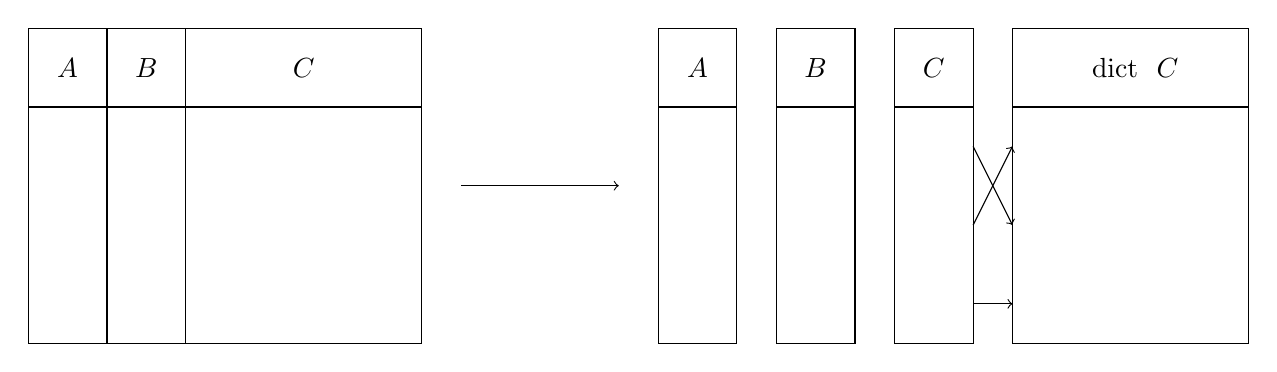
\begin{tikzpicture}[x=0.5cm]
                        \draw
                        (0, 0) -- (10, 0) -- (10, -4) -- (0, -4) -- cycle
                        (0, -1) -- (10, -1)
                        (2, 0) -- (2, -4)
                        (4, 0) -- (4, -4);
                        \node at (1, -0.5) {$A$};
                        \node at (3, -0.5) {$B$};
                        \node at (7, -0.5) {$C$};

                        \draw (11, -2) edge[->] (15, -2);
                        \draw
                        (16, 0) -- (18, 0) -- (18, -4) -- (16, -4) -- cycle
                        (16, -1) -- (18, -1)
                        (19, 0) -- (21, 0) -- (21, -4) -- (19, -4) -- cycle
                        (19, -1) -- (21, -1)
                        (22, 0) -- (24, 0) -- (24, -4) -- (22, -4) -- cycle
                        (22, -1) -- (24, -1)
                        (25, 0) -- (31, 0) -- (31, -4) -- (25, -4) -- cycle
                        (25, -1) -- (31, -1)
                        (24, -1.5) edge[->] (25, -2.5)
                        (24, -2.5) edge[->] (25, -1.5)
                        (24, -3.5) edge[->] (25, -3.5);
                        \node at (17, -0.5) {$A$};
                        \node at (20, -0.5) {$B$};
                        \node at (23, -0.5) {$C$};
                        \node at (28, -0.5) {~dict~ $C$};
                    \end{tikzpicture}
                \end{center}
                Each array contains a pair of OID (uniquely identifies an entry) and value for the $i^\text{th}$ attribute.
                Reconstruction is a simple array access in this case.
                Joins are much more efficient, as we no longer have to read all the data.
                \medskip

                The existing equal-join methods;
                \begin{itemize}
                    \itemsep0em
                    \item sort-merge
                        \subitem one of the relations will not fit in cache, likely meaning we have to read into cache multiple times (take smaller of two relations in main memory)
                    \item hash join \hfill bad if the inner relation doesn't fit into cache
                    \item clustered hash join
                        \subitem one pass to generate cache-sized partitions, take each partition and join it with the other relation, and so on, best of the three solutions, but can be bad if the number of partitions exceed the number of cache lines / TLB entries - can lead to cache thrashing
                \end{itemize}
                This can be addressed with \textbf{radix join}, which first partitions one of the relations and ensure that we partition it into partitions such that we have matching partitions based on $B$ bits of the attribute.
                Matching partitions are joined, nested-loop can be done for small ($\leq 8$ tuples) partitions or a hash join for larger partitions, which is $\leq$ L1 cache, L2 cache, or TLB size (with L1 being ideal).
                This avoids thrashing, compared to clustered hash join.
                Saving these cache misses outweighs the cost of performing extra partitions.
            \subsubsection*{Conclusion}
                The cache performance is important and will become more important as main memory grows.
                The key to this is to cluster data (into a cache line); data that is read together should be written and stored together.
                Irrelevant data should be omitted, including pointers and the use of vertical decomposition.
                Partitions should be done to avoid thrashing.
            \subsubsection*{Spatial Data}
                Spatial data is data with any three dimensions; such as points.
                It has queries such as range queries, nearest neighbours, etc.
                Objects near each other should be stored on the same disk page / cache line, however, there isn't an ordering on data in three dimensions (two objects that are close in 1 dimension could be far apart in another).
                \medskip

                This then goes over an example with reducing computation.
                In the example, checking a range on non-uniform (spatial) partitioning is expensive, as there are many irrelevant points.
                The computation is reduced by using several grids of varying detail; if the range covers the majority of a cell it's checked on that level of detail, if not, it's checked on a lower level of detail.
        \subsection*{October 14 - Live Lecture}
            Learned indexing combines machine learning with indexing.
            The same concept of an index applies, but machine learning models aid to accelerate this lookup, for example by learning distributions.
            These models are typically small and simple, such as interpolation - however, they understand distributions better than existing structures such as B trees.
            The primary challenge is that these models need to fit into main memory, or even the cache to be faster.
            \medskip

            The fundamental problem of a join is to join two relations on a shared attribute.
            If one of the iterations is small, you can iterate over the smaller relation and lookup the related element in the larger relation.
            There are typically two phases in a join, with a build (scanning through the smaller relation and building a hash table), and a probe phase where the second input relation is scanned, and the hash table of the first relation is probed for the matching tuple.
            The problem with this is when the hash table is large, leading to a large number of cache misses.
            One solution is to ensure the hash table can be broken into chunks that fit into cache.
            However, if there are too many partitions, the build phase involves many writes into different partitions, leading to many writes into different locations (thus leading to many TLB misses).
            The radix join addresses this by iteratively partitioning into cache. % ?
            \medskip

            The data in a B+ tree exists in the leaves.
            Any other numbers in internal nodes only exist to help guide the search.
            \medskip

            An adjacent block doesn't necessarily mean a short / small seek distance.
            The abstract concept of an adjacent block could also be called a temporally close block; could be short seek distance or based on rotation.
            Note that the platter is rotating constantly, and by the time the head has finished moving, a different block would be under the head, not necessarily one that is physically nearby.
            If data is written together, it will be stored on adjacent (the abstract concept) blocks, which may still be spread over the disk physically.
            \medskip

            When there's indexing in main memory, the performance is so much faster, the index needs much fewer instructions, otherwise it may be faster to just scan.
            On the other hand, on disks, the performance is relatively slower, allowing for more complex indices.
            This applies even for high-throughput devices.
            \medskip

            DBMS doesn't typically bypass the OS, at least not without a custom OS or specific hardware.
            However, it organises its files or data separately, not leaving it to the OS, as well as handling its own cache and database pages (managed by the database system itself).
            Typically, database systems stores the data in and builds on the OS filesystem.
            You can't force the disk to read / write in a specific physical location, but you can help it write in one go.
        \subsection*{2.1 - Solid State Storage}
            Flash disks can be used as secondary storage or as a caching layer, with the main advantage over traditional disks being that random reads are as fast as sequential reads.
            Disadvantages are slower random writes and a limited number of write cycles.
            Data is organised in pages, which is organised in \textbf{flash blocks}.
            Similar to RAM, the time to retrieve a page isn't related to the location.
            The internals of a flash package are as follows;
            \begin{center}
                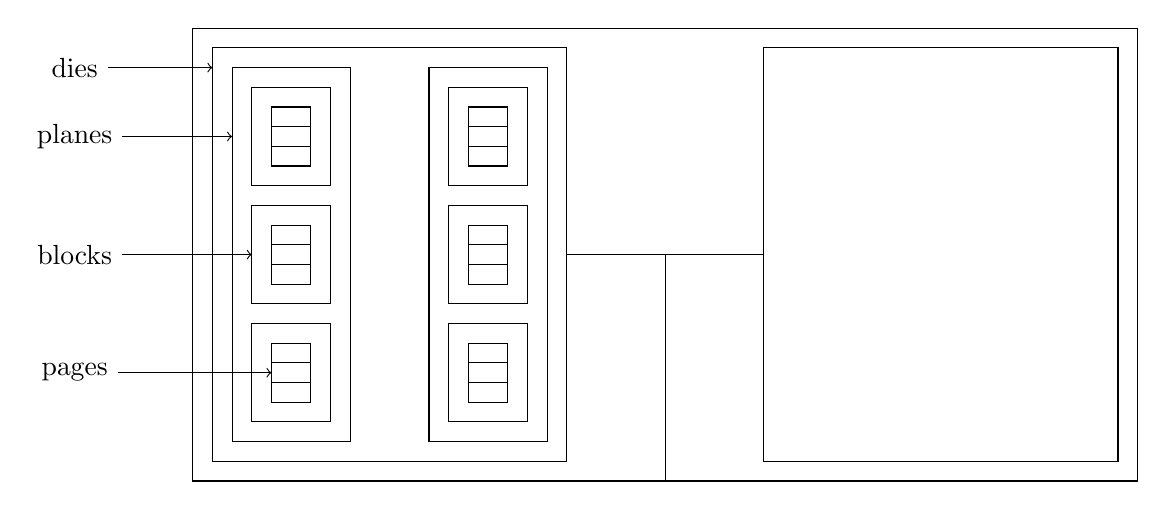
\begin{tikzpicture}[x=0.25cm, y=0.25cm]
                    \node (d) at (-10, 2) {dies};
                    \node (pl) at (-10, -1.5) {planes};
                    \node (b) at (-10, -7.5) {blocks};
                    \node (pa) at (-10, -13.5) {pages};

                    \draw
                    (d) edge[->] (-3, 2)
                    (pl) edge[->] (-2, -1.5)
                    (b) edge[->] (-1, -7.5)
                    (pa) edge[->] (0, -13.5);

                    \draw
                    (-4, 4) -- (44, 4) -- (44, -19) -- (-4, -19) -- cycle
                    (-3, 3) -- (15, 3) -- (15, -18) -- (-3, -18) -- cycle
                    (25, 3) -- (43, 3) -- (43, -18) -- (25, -18) -- cycle
                    (15, -7.5) -- (25, -7.5)
                    (20, -7.5) -- (20, -19);
                    \foreach \x in {0, 10} {
                        \begin{scope}[shift={(\x, 0)}]
                            \draw (-2, 2) -- (4, 2) -- (4, -17) -- (-2, -17) -- cycle;
                            \foreach \y in {0, -6, -12} {
                                \begin{scope}[shift={(0, \y)}]
                                    \draw
                                    (-1, 1) -- (3, 1) -- (3, -4) -- (-1, -4) -- cycle
                                    (0, 0) -- (2, 0) -- (2, -3) -- (0, -3) -- cycle
                                    (0, -1) -- (2, -1)
                                    (0, -2) -- (2, -2);
                                \end{scope}
                            };
                        \end{scope}
                    };
                \end{tikzpicture}
            \end{center}
            There are many of these within an SSD, which in turn is structured as an interface (either SATA or PCI) connected to the internal CPU which is connected to internal memory and the flash controller, which is connected to many flash packages.
            There are no moving parts, hence no mechanical limitations.
            The flash controller helps to ensure the entire drive degrades at roughly the same rate (wear levelling), preventing the capacity from shrinking.
            The access time depends on the bandwidth of the flash packages, device organisation as well as software efficiency.
            The flash translation layer (FTL) is the firmware that manages the hardware.
            \medskip

            A write involves copying the page we are writing to a new page and then deleting the old page, leading to slower random writes.
            On the other hand, if we do a serial write, we can keep it in memory until we have a full flash page.
            Deletion takes time (and is typically on the block level, rather than page) as the pages are densely packed and a high voltage is required to erase a page, seeping into other pages.
            Blocks are isolated from each other, but pages are not (would waste space).
            \medskip

            As the latency gap between CPU and RAM grew, caches were introduced to bridge the gap.
            Similarly, the gap between RAM and HDD can be bridged with SSMs (solid state memory) as a cache or buffer.
            \medskip

            Today, only flash and PCM (phase change memory) are pursued commercially.
            PCM could be placed below flash in the memory hierarchy as the density is still too low.
            \medskip

            DBMS is traditionally designed around a HDD model (buffer management, etc).
            Transactions are only really there (ACID properties) as we need to run things in parallel (since we're waiting on disk and don't want to block).
            Similarly, query plans are also HDD optimisations in the sense they prefer sequential over random access.
            \medskip

            Flash can either be used to replace HDDs, act as an intermediate layer between HDD and RAM, or be used with HDDs on the same level.
            The correct use depends on the workload, such as the amount of data or how the data is accessed, as well as future trends in terms of density.
            \medskip

            Some uses of SSDs in databases;
            \begin{enumerate}[1.]
                \itemsep0em
                \item \textbf{flash-only OLTP}
                    \smallskip

                    OLTP is dominated by random reads and writes, which is very bad for disks, but much faster on flash.
                    With random writes, when used naively in place of a HDD, the throughput drops substantially over time, with significant variance.
                    \medskip

                    The append / pack algorithm; for an append-only operation, we write sequentially as much as we can.
                    No updates are done in place, but rather the old page is invalidated (after reading the content) and a new page is written.
                    Once we run out of space, we reclaim the space and reorganise the storage and continue to write the pages in append-only.
                    Essentially, random writes are transformed into sequential writes and a garbage collection step takes place (with some overhead).
                    This adapts the properties of the algorithm to the underlying hardware.
                \item \textbf{flash-aided business intelligence (OLAP)}
                    \smallskip

                    These are typically read-only queries, with very few scattered updates and complex queries.
                    There are typically two choices - for freshness, updates are performed in-place (with the queries), whereas for performance, updates are done in batches (separate from queries).
                    However, there may be stale data in the latter case.
                    \medskip

                    Flash can be used as a write cache for analytics.
                    Incoming data is written to the SSD, which is then merged with data from the disks to answer a query.
                    We are only using SSDs where it's beneficial; for random accesses.
                    This essentially buffers updates on flash rather than memory, which is larger, cheaper, and also persistent.
                    Of course, this comes with limitations including avoiding random writes (which we saw how to overcome earlier), as well as a limited number of writes due to endurance issues.
                    \medskip

                    The concept behind \textbf{Materialised Sort-Merge (MaSM)} is that we have a system for large scans of tables (like OLAP) which keeps the data on disk when it does it well, but puts updates (where the performance is poor) on SSDs.
                    The data is then merged when queried.
                \item \textbf{logging on flash + HDD}
                    \smallskip

                    Transaction logging is a major bottleneck.
                    Logs are typically what transactions are to be executed (so it can be redone on a failure), which are small sequential writes.
                    The access pattern for this involves small sequential writes which causes a HDD to incur rotational delays.
            \end{enumerate}
            In general, they can be used as a helper on the memory level (not changing the DBMS), adapt the I/O pattern with small DBMS changes, or to fully change storage management.
        \subsection*{2.2 - In-Memory Databases}
            OLAP deals with large amounts of data (data warehousing / data mining) where we look at the output of operational databases, turn them into historical databases and run large, complex, aggregation queries.
            The queries are long running and deal with a large number of tables, and are mostly read-only (only analysing the business).
            On the other hand, OLTP are primarily transactions, hence many small updates.
            There are very few tables touched, with generated queries (not typically human-written).
            \medskip

            OLAP databases are in the order of petabytes, which need to be stored on disks or similar.
            On the other hand, transactional databases are quite small and not growing much; it's possible to buy a TB of main memory.
            \medskip

            On the \textit{Shore DBMS} prototype, only 4\% of the CPU cycles are spent on actual useful work, whereas the remaining 96\% are spent (equally) on latching, recovery (dealing with the log file), locking, and the buffer pool (reading and writing between main memory and disk).
            To improve the performance, improving overhead in processing (better data structures etc., only improves 4\% of the actual performance).
            However, deploying in main memory gets rid of the buffer pool entirely, leading to a solid improvement in performance.
            \medskip

            We have three choices of solutions;
            \begin{itemize}
                \itemsep0em
                \item \textbf{OldSQL} \hfill legacy RDBMS
                    \smallskip

                    Traditional SQL doesn't scale well in the distributed sense.
                \item \textbf{NoSQL} \hfill give up ACID properties to accelerate performance
                    \smallskip

                    ACID properties and transactions are difficult to scale out.
                    Also gives up SQL; the SQL is translated at compile time to a sequence of low level operations (difficult to do).
                    High level queries are also good for abstraction.
                    Giving up data consistency can also be a big issue with NoSQL.
                    \medskip

                    This is appropriate for non-transactional systems, without shared state, and single record transactions that are commutative.
                \item \textbf{NewSQL} \hfill preserves SQL and ACID
                    \smallskip

                    This has both SQL and ACID, and performance and scalability is provided through modern software architecture.
                    It requires solutions for the following, all of which are large sources of overhead;
                    \begin{itemize}
                        \itemsep0em
                        \item \textbf{traditional record level locking} \hfill timestamp order
                        \item \textbf{buffer pool overhead} \hfill removed when moved to main memory
                        \item \textbf{latching for shared data structures} \hfill single-threading for small operations
                        \item \textbf{write-ahead logging} \hfill how to address failure
                    \end{itemize}
            \end{itemize}
            The example we're going to use for NewSQL is \textit{VoltDB}.
            It's all in main-memory (no buffer pool), small single threaded transaction (no concurrency, hence no locks or latches required), and has durability and availability through copies (redundancy) - therefore no traditional log is required.
            Now the 95\% of the cycles are for useful work (with the remainder still being used for some locking).
            \textit{VoltDB} currently runs a subset of SQL, on clusters with LAN and WAN replication.
            It can scale to 384 cores.
            The only locking involved is for multi-partition operations.
            \medskip

            For each of the solutions, only NewSQL is suitable for new OLTP;
            \begin{itemize}
                \itemsep0em
                \item OldSQL is too slow and doesn't scale
                \item NoSQL lacks consistency guarantees and has no language to express queries on a high level (difficult to use)
                \item NewSQL is fast, scalable, consistent, and supports a high level language
            \end{itemize}
            There is a partition per physical CPU core, hence each physical server typically has multiple \textit{VoltDB} partitions.
            Tables can either be \textbf{partitioned} or \textbf{replicated}.
            The former has a single column acting as the partitioning key, allowing rows to be spread across all partitions by the partition column.
            This is better for data with a high modification frequency (transactional data) as it reduces the amount of data being touched.
            On the other hand, the latter has all rows existing in \textbf{all} partitions and is better for mostly static data.
            \medskip

            Similarly, there are also two types of work, which are both ACID.
            Single-partition work happens within a single partition (and requires no locking as it's in a single thread) and is more suitable for the majority of transactional work.
            On the other hand, multi-partition work where we have queries that touch multiple partitions.
            \medskip

            Consider the following ``schema'', where we have three partitions (customer IDs 1 and 4 are in partition 1, 2 and 5 in partition 2, and 3 and 6 in partition 3);
            \begin{lstlisting}
                table orders (partitioned):
                    customer_id (partition key)
                    order_id
                    product_id

                table products (replicated):
                    product_id
                    product_name
            \end{lstlisting}
            Examples of queries are;
            \begin{itemize}
                \itemsep0em
                \item ~select count(*) from orders where customer\_id = 5~ \hfill single (p2)
                \item ~select count(*) from orders where product\_id = 3~ \hfill multi
                    \subitem multi-partition as we don't partition on ~product\_id~, however it's a read operation and no locking is required
                \item ~insert into orders (customer\_id, order\_id, product\_id) values (3,302,2)~ \hfill single (p3)
                    \subitem single-partition if all the values fit in the same partition
                \item ~update products set product\_name = 'spork' where product\_id = 3~ \hfill multi
                    \subitem updating replicated data requires some locking
            \end{itemize}
            In each partition there is a work queue where the queries are coming in.
            There is data for the table and the indices, and a single execution engine which executes requests sequentially - once again, no locking is required as there is no parallelism.
            \medskip

            The database is constructed from the schema (DDL), the work (Java stored procedures), and the project containing users, groups, and partitioning.
            The \textit{VoltCompiler} creates an application catalogue distributed to all machines.
            All access is via Java stored procedures, a single invocation is a transaction that is committed on success, limiting round trips between the DB and the application.
            Communication with the client is asynchronous.
            \medskip

            This scales by adding more machines (or more RAM for more main memory).
            There is high availability from K-safety for redundancy, and snapshots are available, either scheduled, continuous, or on demand (which can be spooled to a data warehouse).
            \medskip

            Due to the asynchronous calls, invocations are sent and responses are pulled from the server, allowing a single client to generate more than 100K transactions per second (TPS) - the client will behave synchronously if required.
            \begin{lstlisting}
                traditional:
                  salary = get_salary(employee_id);
                VoltDB:
                  callProcedure(asyncCallback, "get_salary", employee_id);
            \end{lstlisting}
            However, it doesn't support client-side transaction control (the client cannot perform a rollback) - a stored procedure will commit if it's successful and rollback otherwise.
            The procedure can can call for rollback.
            \medskip

            The lack of concurrency can be beneficial, but it's also important to ensure that any single query is short (transactions should execute in microseconds).
            `Inventory' type applications benefit from this.
            Since locking doesn't have to be considered, dead-locks aren't a concern either.
            As other transactions wait for the running transaction to complete, nothing intensive should be done in a stored procedure (requesting web pages, etc.) - this is useful for OLTP but not OLAP.
            This is optimised for throughput, not latency.
            \medskip

            A subset of SQL is supported; ~SELECT~, ~INSERT~ (with values), ~UPDATE~, and ~DELETE~.
            Aggregations such as ~AVG~, ~COUNT~, ~MAX~, ~MIN~, and ~SUM~ are also supported.
            Functionality will be added over time, but can be done in Java already.
            The execution plan is created at compile time (can be analysed), but may lead to performance issues if there's a drastic change to the cardinality of data (recompile and redeploy in this case)
        \subsection*{October 18 - Live Lecture}
            With SSDs, each page has a limited number of write cycles (around 3,000 per page).
            However, we cannot write to a specific page directly anyways, as this abstracted away by the firmware.
            One important thing to keep in mind is that due to this limitation on SSDs, there may be issues when replacing a HDD for a write-heavy workload.
            Wear-levelling attempts to spread the writes evenly (as much as possible).
            To minimise writes, we should pack writes to be in the sizes of pages.
            When we scan (read sequentially), we are typically limited by the bandwidth of the connection rather than the devices.
            \medskip

            The need for transactions comes from the use of concurrency, which is in place to keep the CPU busy (in traditional databases).
            However, this is not a concern in \textit{VoltDB} as operations are done in serial.
            Locks are to separate user transactions (and protects database contents during entire transactions) and latches are used to separate threads (and protects in-memory data structures during critical sections).
            \medskip

            A concrete example for a fine-grained index versus a coarse-grained one is as follows.
            The former would index every element of an array whereas the latter could take a bunch of entries and index on that; once you're in the `bunch', you still have to perform a scan within it.
            This reduces the complexity by reducing the number of items indexed.
            \medskip

            While \textit{VoltDB} could be constrained by the network bandwidth, however it would likely not reach a bottleneck as the operations are very small (OLTP).
            Additionally, we can't increase transactions indefinitely as it still takes time to process (CPU would be overwhelmed first).
            \medskip

            Append-pack requires more space on the SSD as there is redundant data.
            There is garbage collection to run over the data and pack it together, similar to how defragmentation works.
            There will be some extra work to do (to check whether the page is valid), however overall it's fast enough.
        \subsection*{3 - Graph Databases}
            The example in this lecture will use \textit{Neo4j}, other examples include \textit{OrientDB}, \textit{InfiniteGraph}, and \textit{AllegroGraph}.
            A graph database is a fundamentally different model from traditional relational databases, where we have nodes and relationships between the nodes.
            \medskip

            Graph databases are fairly powerful (and as general as RDBMS, with a fairly direct correspondence between them for translation).
            Works very well if they fit in the main memory of the machine.
            Graph queries check which nodes are connected together.
            Additionally, it's easy to query and scales well on one machine.
            However, scaling out (to multiple machines) is quite difficult - we have graph queries that query relationships between nodes, however this may lead to querying different machines.
            \medskip

            A graph is an abstract representation of a set of objects, with pairs of these objects (also known as vertices or nodes) connected by links (also referred to as edges, arcs, or relationships).
            The different types of graphs are as follows;
            \begin{itemize}
                \itemsep0em
                \item \textbf{undirected} \hfill no indication of direction
                    \begin{center}
                        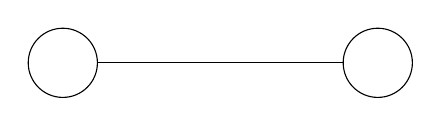
\begin{tikzpicture}
                            \node[state] (a) at (0, 0) {};
                            \node[state] (b) at (4, 0) {};
                            \draw (a) -- (b);
                        \end{tikzpicture}
                    \end{center}
                \item \textbf{directed} \hfill indication of direction, obviously
                    \begin{center}
                        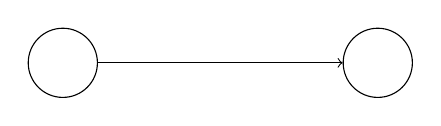
\begin{tikzpicture}
                            \node[state] (a) at (0, 0) {};
                            \node[state] (b) at (4, 0) {};
                            \draw (a) edge[->] (b);
                        \end{tikzpicture}
                    \end{center}
                \item \textbf{pseudo} \hfill only one relationship, pointing to itself
                    \begin{center}
                        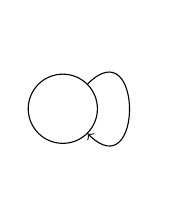
\begin{tikzpicture}
                            \node[state] (a) at (0, 0) {};
                            \draw (a) edge[->, loop, out=45, in=-45, distance=1cm] (a);
                        \end{tikzpicture}
                    \end{center}
                \item \textbf{multi} \hfill multiple relationships between nodes
                    \begin{center}
                        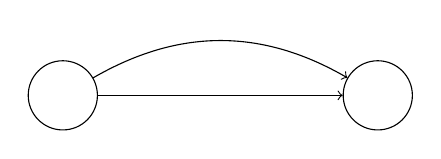
\begin{tikzpicture}
                            \node[state] (a) at (0, 0) {};
                            \node[state] (b) at (4, 0) {};
                            \draw
                            (a) edge[->] (b)
                            (a) edge[->, bend left=30] (b);
                        \end{tikzpicture}
                    \end{center}
                \item \textbf{hyper} \hfill multiple outgoing relationships
                    \begin{center}
                        \begin{tikzpicture}
                            \node[state] (a) at (0, 0) {};
                            \node[state] (b0) at (4, 2) {};
                            \node[state] (b1) at (4, 0) {};
                            \node[state] (b2) at (4, -2) {};
                            \draw
                            (a) edge[->] (b0)
                            (a) edge[->] (b1)
                            (a) edge[->] (b2);
                        \end{tikzpicture}
                    \end{center}
                \item \textbf{weighted} \hfill associated weight with the relationship
                    \begin{center}
                        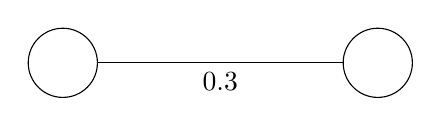
\begin{tikzpicture}
                            \node[state] (a) at (0, 0) {};
                            \node[state] (b) at (4, 0) {};
                            \draw (a) edge[below] node{$0.3$} (b);
                        \end{tikzpicture}
                    \end{center}
                \item \textbf{labelled} \hfill labels for nodes and relationships
                    \begin{center}
                        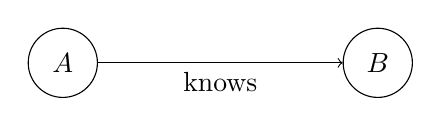
\begin{tikzpicture}
                            \node[state] (a) at (0, 0) {$A$};
                            \node[state] (b) at (4, 0) {$B$};
                            \draw (a) edge[->, below] node{knows} (b);
                        \end{tikzpicture}
                    \end{center}
                \item \textbf{property}
                    \begin{center}
                        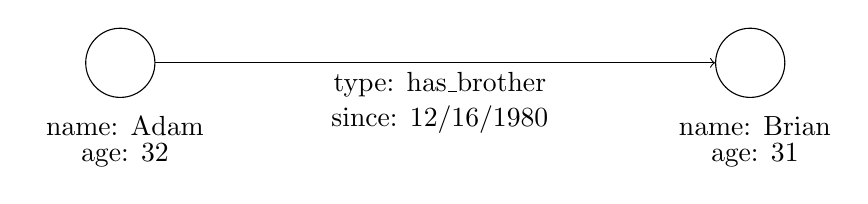
\begin{tikzpicture}
                            \node[state] (a) at (0, 0) {};
                            \node[state] (b) at (8, 0) {};
                            \draw (a) edge[->, below] node{\shortstack{~type: has\_brother~\\~since: 12/16/1980~}} (b);
                            \node at (0, -1) {\shortstack{~name: Adam~\\~age: 32~}};
                            \node at (8, -1) {\shortstack{~name: Brian~\\~age: 31~}};
                        \end{tikzpicture}
                    \end{center}
                    This is the closest to what \textit{Neo4j} uses.
                    In this property graphs, nodes and relationships can have arbitrary properties, typically key-value pairs.
            \end{itemize}
            Consider a many-to-many relationship in a typical RDBMS, in this example we have ~people~, ~departments~, and ~department\_member~ tables (where the latter joins the former two).
            In a graph model, there could simply be relationships from each entry in ~people~ to each of the entries in ~department~, with a ~belongs\_to~ (or similar) relationship.
            This eliminates the requirement for joins, which can be complicated if many joins are involved.
            A graph data model can be easily constructed by writing down the entities involved as nodes and then creating relationships between them.
            From here, properties (key-value pairs) can be added in to the nodes and relationships.
            It's generally quite similar to ER mapping, but we don't need to consider cardinality.
            \medskip

            A graph databases has an explicit graph structure, with each node knowing its adjacent nodes (has links to) - which ideally lives in the same machine.
            Each node has indices for its neighbouring nodes to allow for fast access; the cost for a local step remains the same even if the number of nodes increase, however it can become slower if the hops are to different machines (network latency).
            \medskip

            To translate to \textit{Neo4j};
            \begin{itemize}
                \itemsep0em
                \item each entity table is a label on nodes
                \item each row in an entity table is a node, with the columns being node properties
                \item add unique constraints for business primary keys and indices for attributes which are frequently looked up
            \end{itemize}
            A node can have relationships and properties.
            A relationship has a start and end node, has a relationship type which is uniquely identified by a name, and can have properties.
            Property keys are strings, whereas property values can either be a primitive type or an array of a primitive type.
            A path in \textit{Neo4j} is one or more nodes with connection relationships that can be retrieved as a query or the result of a traversal.
            Querying this in a traditional relational database could be very inefficient as you may end up querying tables multiple times.
            \medskip

            Cypher is very similar to SQL, but for graphs.
            It is a declarative (no need to tell it how to retrieve things), pattern-matching language.
            Some examples are as follows;
            \begin{itemize}
                \itemsep0em
                \item retrieves all pairs of nodes that are connected with a relationship; doesn't specify \textbf{what} relationship
                    \begin{lstlisting}
                        START a=node(*) // now optional
                        MATCH (a)-->(b) // a and b are just placeholders (connection is important)
                        RETURN a, b;
                    \end{lstlisting}
                \item find all nodes with an outgoing relationship and get a specific property (~name~ in this case) - no set property schema (similar to document databases), just ensure no name collisions
                    \begin{lstlisting}
                        START a=node(*)
                        MATCH (a)-->()
                        RETURN a.name;
                    \end{lstlisting}
                \item find all actors which have acted in a movie
                    \begin{lstlisting}
                        START a=node(*)
                        MATCH (a)-[:ACTED_IN]->(m)
                        RETURN a, m;
                    \end{lstlisting}
                \item with paths, note that ~(a)-->(b)-->(c)~ is different from ~(a)-->(b)<--(c)~
                \item get actor and director names for movie titles;
                    \begin{lstlisting}
                        START a=node(*)
                        MATCH (a)-[:ACTED_IN]->(m)<-[:DIRECTED]-(d)
                        // equivalent to the following (since m is named);
                        // MATCH (a)-[:ACTED_IN]->(m), (m)<-[:DIRECTED]-(d)
                        // MATCH (a)-[:ACTED_IN]->(m), (d)-[:DIRECTED]->(m)
                        RETURN a.name, m.title, d.name;
                    \end{lstlisting}
                \item sorting and limit can also be done (same as SQL) (count movies actors and directors have worked together in);
                    \begin{lstlisting}
                        START a=node(*)
                        MATCH (a)-[:ACTED_IN]->(m)<-[:DIRECTED]-(d)
                        RETURN a.name, d.name, count(*) AS count
                        ORDER BY(count) DESC
                        LIMIT 5;
                    \end{lstlisting}
                \item aggregations
                    Aggregations can also be done in a similar way;
                    \begin{itemize}
                        \itemsep0em
                        \item ~count(x)~ \hfill add number of occurrences
                        \item ~min(x)~ \hfill get lowest value
                        \item ~max(x)~ \hfill get highest value
                        \item ~avg(x)~ \hfill average of numeric values
                        \item ~collect(x)~ \hfill collects into an array (`transposes' a column)
                    \end{itemize}
                    An example of this is as follows, where we get the actors and directors who have worked together (and an array of movie titles);
                    \begin{lstlisting}
                        START a=node(*)
                        MATCH (a)-[:ACTED_IN]->(m)<-[:DIRECTED]-(d)
                        RETURN a.name, d.name, collect(m.title);
                    \end{lstlisting}
                \item find a specific node (query all nodes); in this example we search for the name ~John Smith~
                    \begin{lstlisting}
                        START n=node(*)
                        WHERE has(n.name) AND n.name = "John Smith"
                        RETURN n;
                    \end{lstlisting}
                    Note that the ~has(n.name)~ part ensures that the ~name~ property exists.
                    This is required as we don't know that every node has this property.
                \item create a new ~KNOWS~ relationships between actors and directors who have worked together
                    \begin{lstlisting}
                        START a=node(*)
                        MATCH (a)-[:ACTED_IN|DIRECTED]->()<-[:ACTED_IN|DIRECTED]-(b)
                        CREATE UNIQUE (a)-[:KNOWS]->(b);
                    \end{lstlisting}
                \item paths can have variable lengths - the following example matches the following paths; ~(a)-->(b)~, ~(a)-->()-->(b)~, or ~(a)-->()-->()-->(b)~
                    \begin{lstlisting}
                        START a=node(*)
                        MATCH (a)-[*1..3]->(b)
                        RETURN a, b;
                    \end{lstlisting}
                    This is quite difficult to represent in a traditional relational database.
                    An application of this is as follows, where we try to find the friends-of-friends of ~John Smith~;
                    \begin{lstlisting}
                        MATCH (john)-[:KNOWS*2]->(fof)
                        WHERE has(john.name) AND john.name = "John Smith"
                        RETURN DISTINCT fof.name;
                    \end{lstlisting}
                \item this searches for movies in which ~Keanu Reeves~ played ~Neo~ - note that it also shows that properties can be sets
                    \begin{lstlisting}
                        MATCH (actor)-[r:ACTED_IN]->(movie)
                        WHERE "Neo" IN r.roles AND actor.name = "Keanu Reeves"
                        RETURN DISTINCT movie.title;
                    \end{lstlisting}
                \item actors who worked with ~Gene Hackman~ and are also directors (constraints can also be patterns)
                    \begin{lstlisting}
                        MATCH (gene)-[:ACTED_IN]->(movie)<-[:ACTED_IN]-(n)
                        WHERE (n)-[:DIRECTED]->() AND gene.name = "Gene Hackman"
                        RETURN DISTINCT n.name;
                    \end{lstlisting}
                \item creating a node and adding properties % not sure if it should be a.tagline or movie.tagline, but whatever
                    \begin{lstlisting}
                        CREATE ({title:"Mystic River", released:1993}); // create new node

                        // similar to SQL, adding a tagline
                        START movie=node(*)
                        MATCH (movie)
                        WHERE movie.title = "Mystic River"
                        SET movie.tagline = "Lorem Ipsum"
                    \end{lstlisting}
                \item creating a relationship
                    \begin{lstlisting}
                        CREATE UNIQUE (kevin)-[:ACTED_IN {roles:["Sean"]}]->(movie)
                        WHERE movie.title = "Mystic River" AND kevin.name = "Kevin Bacon";
                    \end{lstlisting}
                \item deleting relationships (remove all relationships for ~John Smith~)
                    \begin{lstlisting}
                        MATCH (a)-[r]->()
                        WHERE a.name = "John Smith"
                        DELETE r;
                    \end{lstlisting}
                    Similarly, if we wanted to delete ~John Smith~ and relationships (regardless of whether any exist);
                    \begin{lstlisting}
                        MATCH (a)-[r?]->()
                        WHERE a.name = "John Smith"
                        DELETE r, a;
                    \end{lstlisting}
            \end{itemize}
\end{document}